%----------------------------------------------------------------------------------------
% (c) 2019 eta systems GmbH.
% github.com/eta-systems
% 
% LaTeX Template for SG-Mini Testbench Report
% 
% This work is licensed under a Creative Commons Attribution 4.0 International License.
% https://creativecommons.org/licenses/by/4.0/
%----------------------------------------------------------------------------------------

%----------------------------------------------------------------------------------------
%	PACKAGES AND DOCUMENT CONFIGURATIONS
%----------------------------------------------------------------------------------------
\documentclass[a4paper,12pt]{article}

\usepackage{siunitx}         	% si{} units for 12.4\si{\Volt}
\usepackage{graphicx}  			% graphics
\usepackage{amsmath}  			% for certain math elements
\usepackage[T1]{fontenc} 		% fonts
\usepackage[utf8]{inputenc}
\usepackage[yyyymmdd]{datetime}
\renewcommand{\dateseparator}{-}

% document margins - include before fancyhdr
\usepackage[includeheadfoot,left=2cm,top=2cm,right=2cm,bottom=1.6cm]{geometry}
\geometry{
	a4paper
}

\usepackage{fancyhdr} 			% header / footer
\fancyhead[L]{\textsf{\rightmark}}
\fancyhead[R]{\textsf{\leftmark}}
\renewcommand{\headrulewidth}{0.4pt} % line under the header

\fancyfoot[L]{\textsf{\thepage}}
\fancyfoot[C]{}
\fancyfoot[R]{
	{\fontfamily{cmss}\selectfont
		$\eta$ eta systems
	}
}
\renewcommand{\footrulewidth}{0.4pt} % line under the footer
\pagestyle{fancy}               % use the custom headers throughout the document

% \setlength\parindent{0pt} % remove paragraph indentation

%----------------------------------------------------------------------------------------
%	Frontpage
%----------------------------------------------------------------------------------------

\title{Silentgenerator Mini (SG-Mini) \\ Factory Line Report }

\author{
	{\fontfamily{cmss}\selectfont
		GmbH
		\makebox[-2cm][r]{\raisebox{-2ex}{
\includegraphics[height=1.6cm]{graphics/logo.png}}}
	}
}

\begin{document}

\maketitle

\begin{center}
	\begin{tabular}{l r}
		Serial Number & REPLACE-SERIAL-NUMBER \\
		Date of Test: & \today \\
		Operator & REPLACE-OPERATOR \\
		Script Version: & REPLACE-SCRIPT-VERSION \\
	\end{tabular}
\end{center}

\clearpage

%----------------------------------------------------------------------------------------
%	Test Procedure
%----------------------------------------------------------------------------------------

\section{Test Procedure}

Testing with a voltage of ${REPLACE-VOLTAGE-INPUT \si{V}}$.


% may look too wide with placeholder values
% once replaced with shorter numerical values the table will be smaller
\begin{center}
	\begin{table}[]
		\begin{tabular}{|l|l|l|l|l|l|}
			\hline
			\textbf{Symbol} & \textbf{Ratings}             & \textbf{min}                & \textbf{typ}              & \textbf{max}                & \textbf{Unit} \\ \hline
			${V_{in}}$      & Input Voltage                &                             & ${REPLACE-VOLTAGE-INPUT}$ &                             & ${\si{V}}$    \\ \hline
			${I_{out}}$     & Output Current               & ${REPLACE-CURRENT-OUT-MIN}$ &                           & ${REPLACE-CURRENT-OUT-MAX}$ & ${\si{A}}$    \\ \hline
			n               & Number of measurement points &                             & ${REPLACE-DPOINTS}$       &                             &               \\ \hline
		\end{tabular}
	\end{table}
\end{center}


%----------------------------------------------------------------------------------------
%	Results of Efficency Test
%----------------------------------------------------------------------------------------

\section{Efficiency of DC/DC Converter}

\begin{figure}[h]
\begin{center}
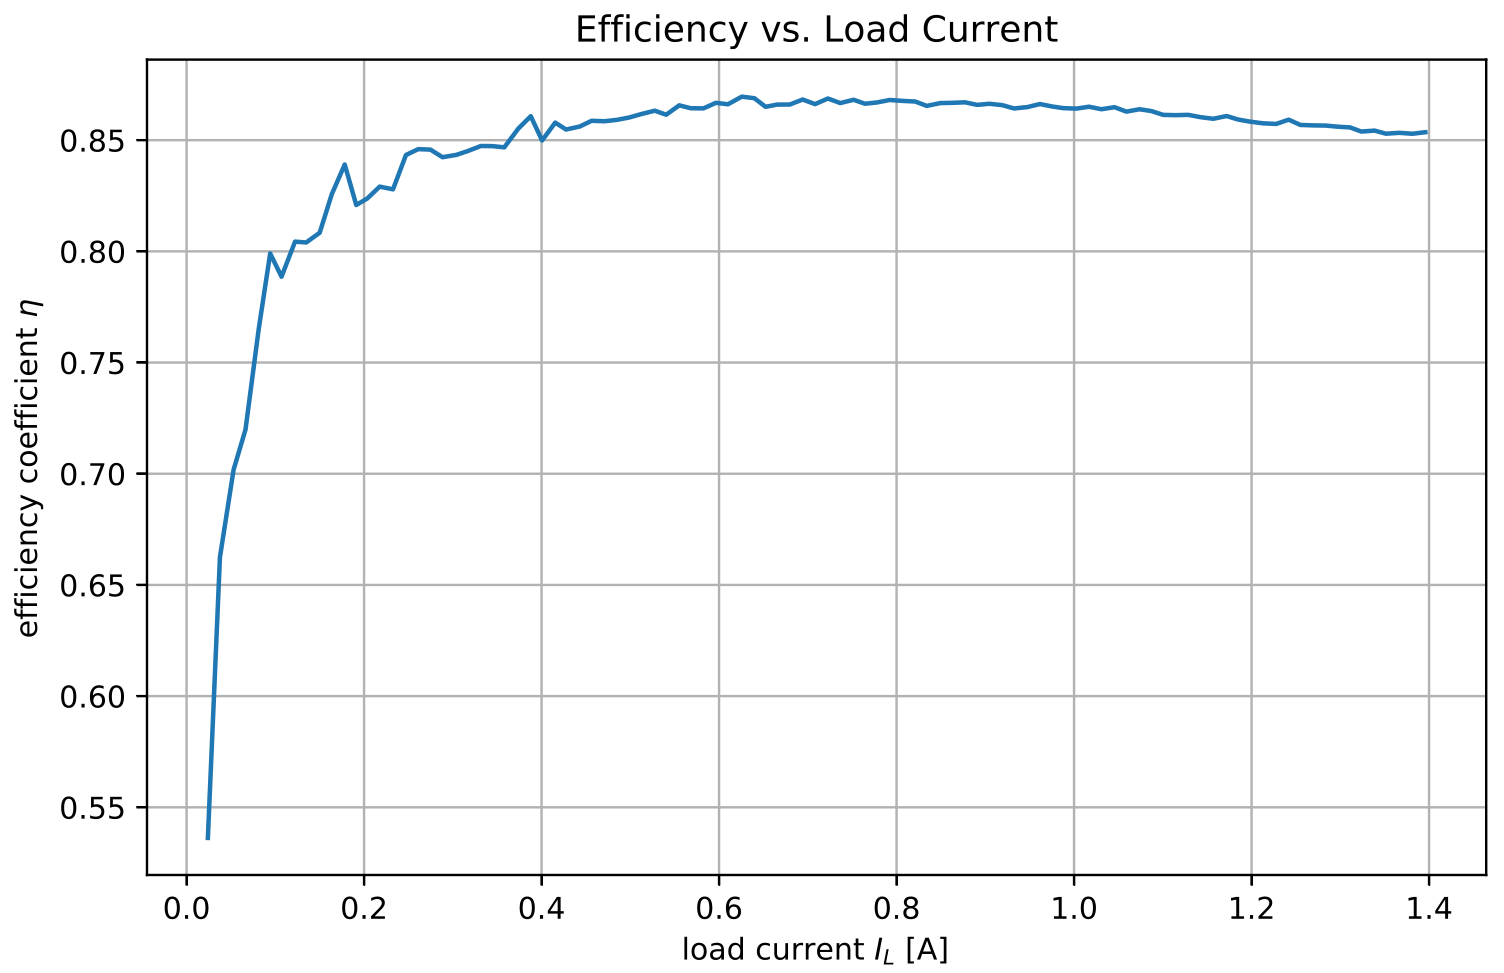
\includegraphics[width=0.70\textwidth]{graphics/Efficiency_vs_LoadCurrent.png}
\caption{Graph showing efficiency in function of load current.}
\end{center}
\end{figure}



\end{document}